

\documentclass[a4paper]{article}

\usepackage{amsmath}
\usepackage{hyperref}
\usepackage{biblatex}
\usepackage{enumerate}
\usepackage{graphicx}
\usepackage{stmaryrd}
\usepackage[dvipsnames]{xcolor}
\usepackage{listings}
\usepackage{caption}
\usepackage{subcaption}
\usepackage{booktabs}
\usepackage{float}

\addbibresource{refs.bib}

\begin{document}

\author{Ola Bratt \\
  \href{mailto:ola.bratt@gmail.com}{ola.bratt@gmail.com}
  \and
  Patrick Attimont \\
  \href{patrickattimont@gmail.com}{patrickattimont@gmail.com}
}

\title{DAT565/DIT407 Assignment 6}
\date{2024-02-xx}

\maketitle

This paper is addressing the assignment 6 study queries within the \emph{Introduction to Data Science \& AI} course, DIT407 at 
the University of Gothenburg and DAT565 at Chalmers. The main source of information for this project
is derived from the lectures and Skiena~\cite{Skiena:2024}. Assignment 6 is about neural networks.

\section*{Problem 1: The dataset}

The dataset consists of 60,000 training images and 10,000 test images. 
Each image is a 28x28 pixel grayscale image. 
The images are labeled with the corresponding digit. 
A random set of the images are shown in figure~\ref{fig:mnist_images}.



\begin{figure}[H]
  \begin{center}
    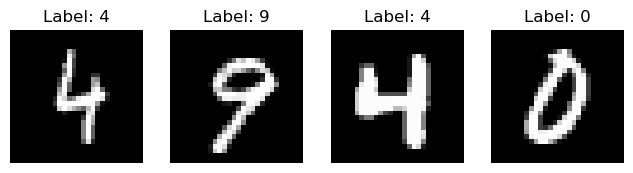
\includegraphics[width=\textwidth]{ola/mnist_images.png}
    \caption{MNIST images}
    \label{fig:mnist_images}
  \end{center}
\end{figure}

\section*{Problem 2: Single hidden layer}

The neural network with a single hidden layer has 784 (28*28) input nodes, 300 hidden nodes, and 10 output nodes.
The activation function is ReLU for the hidden layer with a batch normalization and logarithmic softmax for the output layer.

\begin{verbatim}
  Epoch [1/10], Training Loss: 0.2200, Test Loss: 0.1065, Test Accuracy: 0.9695
  Epoch [2/10], Training Loss: 0.1057, Test Loss: 0.0921, Test Accuracy: 0.9725
  Epoch [3/10], Training Loss: 0.0768, Test Loss: 0.0728, Test Accuracy: 0.9765
  Epoch [4/10], Training Loss: 0.0613, Test Loss: 0.0666, Test Accuracy: 0.9793
  Epoch [5/10], Training Loss: 0.0497, Test Loss: 0.0643, Test Accuracy: 0.9791
  Epoch [6/10], Training Loss: 0.0421, Test Loss: 0.0639, Test Accuracy: 0.9798
  Epoch [7/10], Training Loss: 0.0355, Test Loss: 0.0628, Test Accuracy: 0.9811
  Epoch [8/10], Training Loss: 0.0309, Test Loss: 0.0569, Test Accuracy: 0.9823
  Epoch [9/10], Training Loss: 0.0279, Test Loss: 0.0616, Test Accuracy: 0.9796
  Epoch [10/10], Training Loss: 0.0225, Test Loss: 0.0590, Test Accuracy: 0.9816
\end{verbatim}

Accuracy for single hidden layer: 0.9816

\begin{figure}[H]
  \begin{center}
    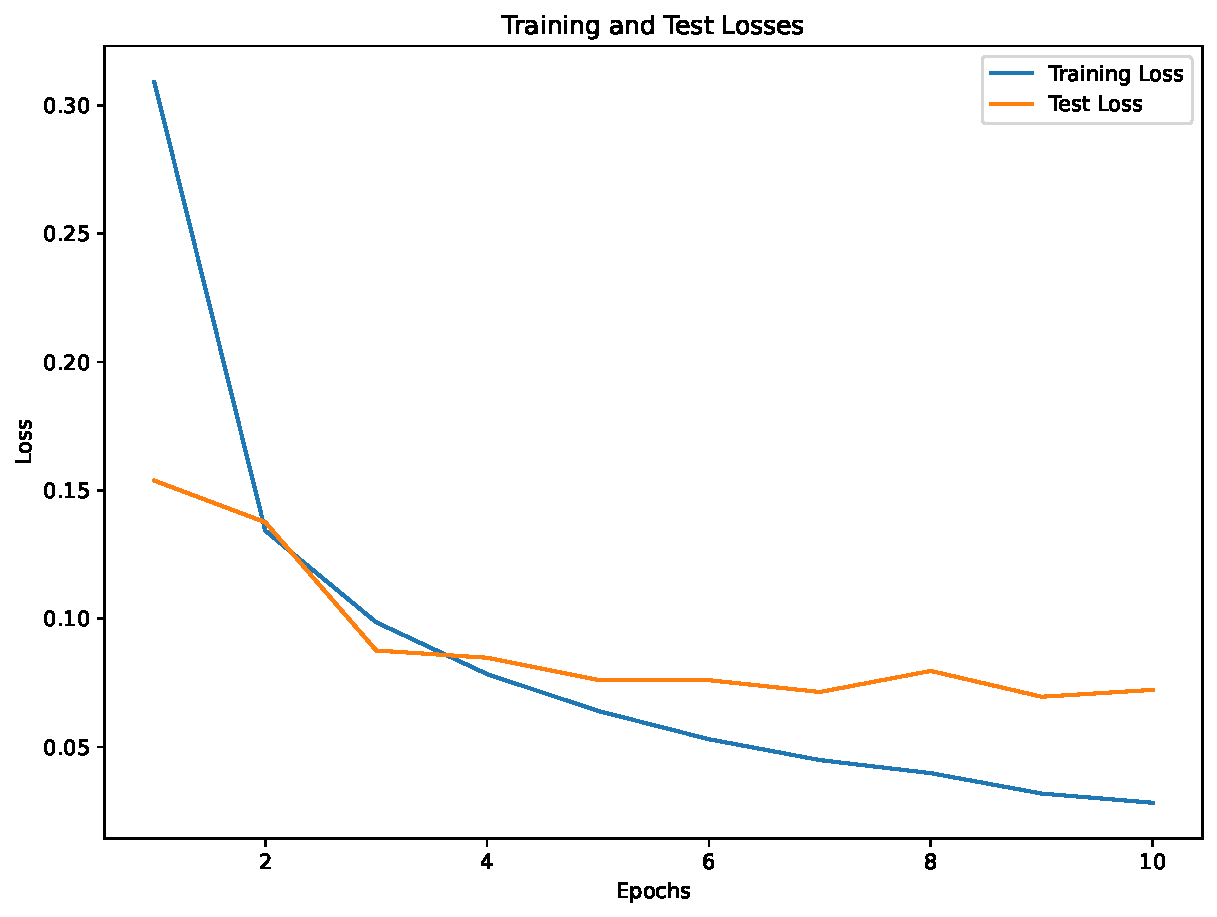
\includegraphics[width=\textwidth]{ola/single_hidden_layer.pdf}
    \caption{Single hidden layer}
    \label{fig:single_hidden_layer}
  \end{center}
\end{figure}

\section*{Problem 3: Two hidden layers}

Accuracy for two hidden layers: 0.9855


\begin{figure}[H]
  \begin{center}
    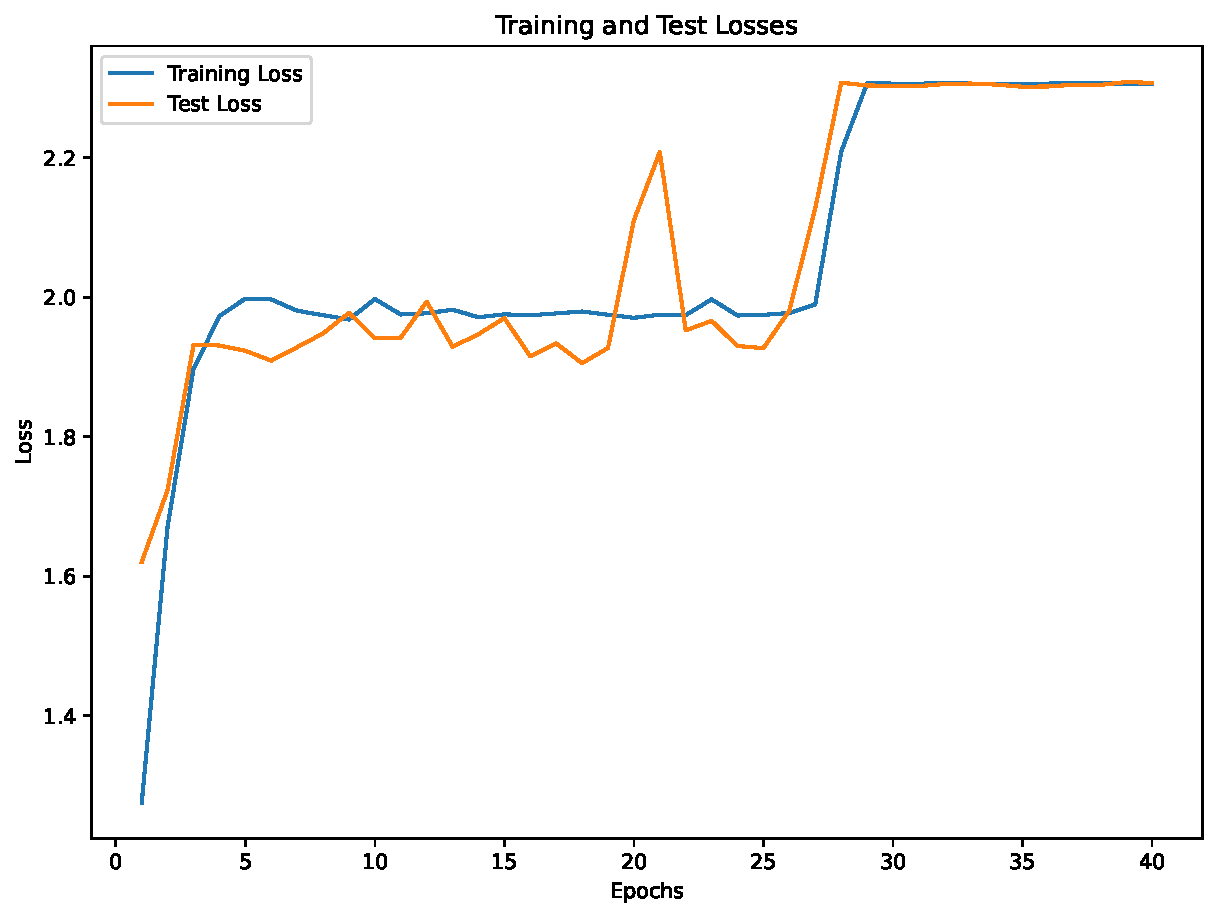
\includegraphics[width=\textwidth]{ola/two_hidden_layer.pdf}
    \caption{Two hidden layers}
    \label{fig:two_hidden_layers}
  \end{center}
\end{figure}

\section*{Problem 4: Convolutional neural network}

Accuracy for convolutional neural network: 0.9929



\begin{figure}[H]
  \begin{center}
    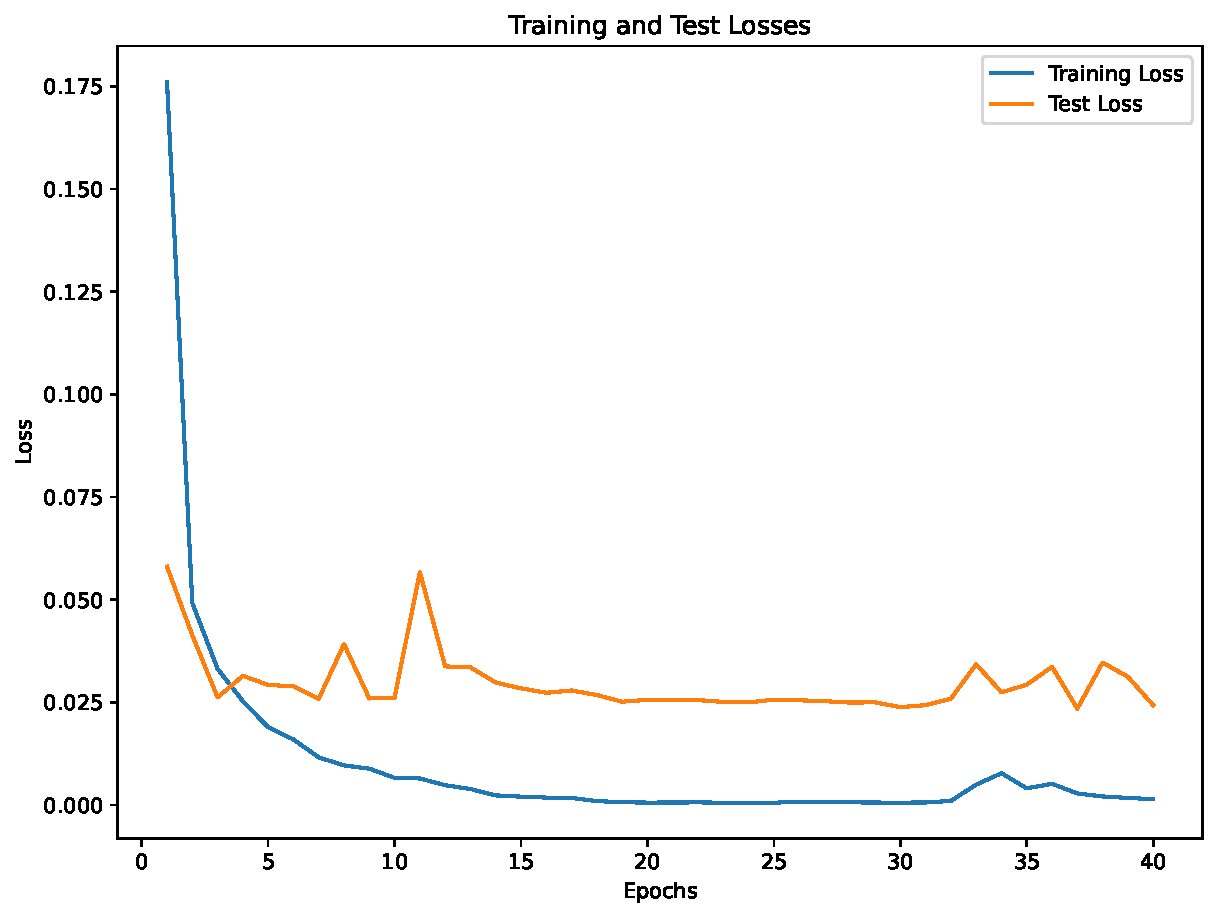
\includegraphics[width=\textwidth]{ola/cnn.pdf}
    \caption{Convolutional neural network}
    \label{fig:convolutional_neural_network}
  \end{center}
\end{figure}


\newpage


\printbibliography

\section*{Appendix: Source Code}

\lstset{
  language=Python,
  basicstyle=\ttfamily,
  commentstyle=\color{OliveGreen},
  keywordstyle=\bfseries\color{Magenta},
  stringstyle=\color{YellowOrange},
  numbers=left,
  basicstyle=\footnotesize,
  breaklines=true,
  postbreak=\mbox{\textcolor{red}{$\hookrightarrow$}\space}
}


\lstinputlisting{ola/assignment6.py}

\end{document}
